\documentclass[main.tex]{subfiles}
\begin{document}
% 5,  part 2
\begin{psec}{5.20}%
Next,
we look at some properties of the square root map.
\begin{enumerate}
\item \label{5.20-1} \statement{
Let $S\in\mathscr{H}$, $T\in{\mathscr H}^+$.
If $S$ commutes with~$T$,
then it commutes with~$\sqrt{T}$.}
This follows from the last part of~\ref{5.19}:
$S$ commutes with all powers of~$T$,
therefore with every $\sr_n(T)$,
therefore with~$\sqrt{T}$.
%
\item \label{5.20-2} \statement{
If $S,T\in\mathscr{H}^+$ and $ST=TS$, then $ST\in{\mathscr H}^+$.}

\noindent \emph{Proof}\  By~\ref{5.12}, $ST\in{\mathscr H}$.
As for the positivity: 
\ref{5.20-1} implies that~$T$ commutes with~$\sqrt{S}$
and, again, that~$\sqrt{S}$ commutes with~$\sqrt{T}$.
Then $ST=\smash{\sqrt{S}^2} \smash{\sqrt{T}^2}
= \smash{\bigl(\sqrt{S}^{\phantom{2}}\sqrt{T}\,\bigr)^2}\in{\mathscr H}^+$
\quad(\ref{5.9}). \xqed
%
\item \label{5.20-3} \statement{
Let $S,T\in\mathscr{H}$, $S\leq T$.
Then $VS\leq VT$ for every~$V$ in~${\mathscr H}^+$
that commutes with~$S$ and with~$T$.}

\noindent \emph{Proof}\  $VS-VT=V(T-S)\in{\mathscr H}^+$,
by~\ref{5.20-2}. \xqed
%
\item \label{5.20-4} \statement{
Let $S,T\in{\mathscr H}^+$, $ST=TS$.
If $S\leq T$, then $S^2 \leq T^2$.}

\noindent \emph{Proof}\ With~\ref{5.20-3}:
$SS\leq ST=TS\leq TT$. \xqed
%
\item \label{5.20-5} \statement{
Let $T\in{\mathscr H}^+$, $V\in\mathscr H$, $TV=VT$.
If $V^2\leq T$, then $V\leq \sqrt{T}$.}

\noindent\emph{Proof}\  We may assume $\|T\|=1$.
Let~$q_n$ be as in~\ref{5.18} and~\ref{5.19},
so that $q_n(I-T)\rightarrow I-\sqrt{T}$.
We are done if $q_n(I-T)\leq I-V$ for all~$n$.
This inequality can be proved inductively.
First: 
\begin{alignat*}{2}
I-V-q_1(I-T) 
& = I-V-{\textstyle \frac{1}{2}}(I-T)  & \\
& = {\textstyle \frac{1}{2}} I - V + {\textstyle \frac{1}{2}} T & \\
& \geq {\textstyle \frac{1}{2}} I - V + {\textstyle \frac{1}{2}} V^2
 &= {\textstyle \frac{1}{2}} (I-V)^2 \geq 0\htam{,}
\end{alignat*}
so $q_1(I-T)\leq I-V$.

Second:  if~$n$ is so that $q_n(I-T)\leq I-V$, then
\begin{alignat*}{2}
2q_{n+1} (I-T) 
& = I-T+(q_n(I-T))^2 & \\
& \relref{\leq}{5.20-4} I-T+(I-V)^2 & \\
& \leq I-V^2+(I-V)^2 & = 2(I-V)
\end{alignat*}
and $q_{n+1} (I-T) \leq I-V$. \xqed
%
\item \label{5.20-6} \statement{
If $T\in{\mathscr H}^+$, then $\smash{\sqrt{T^2}=T}$.}

\noindent \emph{Proof} Put $S:=\smash{\sqrt{T^2}}-T$.
By~\ref{5.20-5}, $T\leq \smash{\sqrt{T^2}}$,
i.e., $S\geq 0$.
Then $ST\geq 0$ according to~\ref{5.20-2}.
But~$ST$ equals $-\frac{1}{2} S^2$.
Hence for all~$x$ in~$H$
\begin{equation*}
\|Sx\|^2 = \left<Sx,Sx\right>=\left<S^2 x,x\right>
=-2\left<STx,x\right>\leq 0\htam{.}
\end{equation*}
It follows that $S=0$, and $\smash{\sqrt{T^2}}=T$. \xqed
\end{enumerate}
\end{psec}
%
%                  5.21
%
\begin{psec}{5.21}{Exercise}
Let $S,T\in{\mathscr H}^+$ be so that $\|Sx\|=\|Tx\|\quad(x\in H)$.
Prove $S=T$.
(Show first that $S^2 = T^2$.)
\end{psec}
%
%                  5.22
%
\begin{psec}{5.22}{Exercise}
(This we need farther on.)
Prove the following.
\begin{enumerate}
\item\label{5.22-1}
If $T\in\mathscr H$ and $0\leq T\leq I$, then $T^2\leq T$.
%
\item\label{5.22-2}
If $T\in\mathscr H$ and $0\leq T\leq I$,
then $\|Tx\|^2\leq \left< Tx,x\right>\quad (x\in H)$.
%
\item\label{5.22-3}
If $S,T\in\mathscr H$ and $0\leq S\leq T\leq I$,
then 
\begin{equation*}
\|Tx-Sx\|^2 \leq \left<Tx,x\right>-\left<Sx,x\right>\qquad (x\in H)\htam{.}
\end{equation*}
\end{enumerate}
\end{psec}
%
%                  5.23
%
\begin{psec}{5.23}{Exercise}
(built upon the previous one)
Let $T\in\mathscr H$, $0\leq T\leq I$
(or: $T\in{\mathscr H}^+$, $\|T\|\leq 1$).
Prove:
\begin{enumerate}
\item\label{5.23-1}
$I\geq T \geq T^2 \geq \dotsb$.
%
\item\label{5.23-2}
$Px:=\lim_{n\ra\infty} T^n x$ exists for all~$x$ in~$H$.

This defines a (linear) map $P\colon H\ra H$.
For each~$x$ in~$H$
we see that $\|x\|\geq\|Tx\|\geq\|T^2 x\|\geq \dotsb$,
so that $\|Px\|\leq \|x\|\quad (x\in H)$
and~$P$ is continuous.
%
\item\label{5.23-3}
$P\in\mathscr H$, $0\leq P \leq T\leq I$.
%
\item\label{5.23-4}
$P=P^2$. (Careful: From $T^n x\ra Px\quad(x\in H)$
it does not immediately follow that $T^{2n} x\ra P^2 x\quad(x\in H)$.
Instead, prove $\left<Px,x\right>=\|Px\|^2$.)

Thus, $P$ is a projection (\ref{5.7}).
%
\item\label{5.23-5}
If $x\in H$ and $Tx=x$,
then $Px=x$.
Conversely,
if $x\in H$ and $Px=x$,
then $\left< Tx,x\right>=\left<x,x\right>$,
so $Tx-x\perp x$,
whence $Tx=x$ (Pythagoras).

$P$ is the projection onto $\left\{ x\colon Tx=x \right\}$.
\end{enumerate}
\end{psec}
%
%                  5.24
%
\begin{psec}{5.24}{Exercise}
(built upon the previous one)
\begin{center}
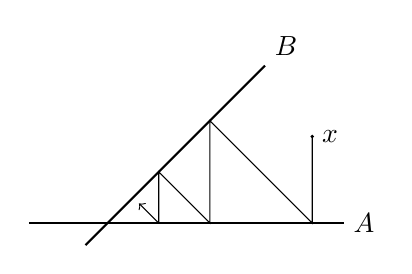
\begin{tikzpicture}
% A:
\draw[line width=.8pt] (-1,0) -- (3,0);
\draw (3,0) node[anchor=west]{$A$};

% B:
\draw[line width=.8pt] (-.28,-.28) -- (2,2);
\draw (2,2) node[anchor=south west]{$B$};

% x:
\draw[fill=black] (2.6,1.1) circle (.4pt);
\draw (2.6,1.1) node[anchor=west]{$x$};

% projections:
\draw (2.6,1.1) -- (2.6,0) -- (1.3,1.3) -- (1.3,0) -- (.65,.65) -- (.65,0);
\draw[->] (.65,0) -- (.4,.25);
\end{tikzpicture}
\end{center}
Let~$A$ and~$B$ be closed linear subspaces of~$H$
with projections~$Q$ and~$R$, respectively.
We consider the sequence
\begin{equation*}
Q,\ RQ,\ QRQ,\ RQRQ,\ \dotsc
\end{equation*}
Prove the following.
\begin{enumerate}
\item\label{5.24-1}
$QRQ\in\mathscr H$, $0\leq QRQ \leq I$.
%
\item\label{5.24-2}
For all $x\in H$ the sequence $QRQx$,  $QRQRQx$, 
$\dotsc$ converges.

Denote its limit by~$Px$.
We now have a map $P\colon H\ra H$.
%
\item\label{5.24-3}
$P$ is the projection onto $A\cap B$.
(If $QRQx=x$, then $x\in Q(H)$, so $Qx=x$.)
%
\item\label{5.24-4}
For every~$x$ the sequence
\begin{equation*}
Qx,\ RQx,\ QRQx,\ RQRQx,\ \dotsc
\end{equation*}
converges to~$Px$.
\end{enumerate}
\end{psec}

\noindent
We begin to get results:
\begin{psec}{5.25}{Lemma}\statement{
Let $\mathscr A$ be a closed subalgebra of~$\mathscr H$.
\begin{enumerate}
\item\label{5.25-1} $\mathscr A$ is a Riesz space
under the ordering of~$\mathscr H$, and 
\begin{equation*}
|T|\ =\ \sqrt{T^2}\qquad(T\in\mathscr A)\htam{.}
\end{equation*}
If $\mathscr B$ is a closed subalgebra of~$\mathscr H$
and $\mathscr B \subseteq \mathscr A$,
then $\mathscr B$ is a Riesz subspace of~$\mathscr A$.
%
\item\label{5.25-2} If $I\in\mathscr A$,
then~$I$ is a unit,
the norm~$\|\cdot\|_I$ is the operator norm,
and~$\mathscr A$ is uniformly complete.
\end{enumerate}
}\end{psec}
\begin{proof}
\begin{enumerate}
\item
It suffices to prove that for $T\in \mathscr A$,
$\smash{\sqrt{T^2}}$ is the supremum of $\{T,-T\}$
in the ordered vector space~$\mathscr A$.
Let $T\in\mathscr A$.
\begin{itemize}
\item  In the final lines of~\ref{5.19}
we have seen that $\sqrt{T}\in\mathscr A$,
\item $\pm T \leq \smash{\sqrt{T^2}}$, 
since $(\pm T)^2\leq T^2$ (\ref{5.20}\ref{5.20-5}).
\item Let $W$ be an upper bound of $\{T,-T\}$ in~$\mathscr A$.
Then $W\geq \frac{1}{2}(T+-T)=0$.
Also, with~\ref{5.20}\ref{5.20-2}, 
$0\leq (W-T)(W+T)=W^2-T^2$,
so that $W^2\geq T^2$ and,
with~\ref{5.20}\ref{5.20-6} and~\ref{5.20}\ref{5.20-5},
$W=\smash{\sqrt{W^2}}\geq\smash{\sqrt{T^2}}$.
\end{itemize}
%
\item \label{5.25-2}
For $T\in\mathscr A$
we see that $|T|^2=T^2$.
Then for all~$x$ in~$H$
\begin{equation*}
\| T x \|\ = \|\, |T|x\, \|\htam{,}
\end{equation*}
since
$\|Tx\|^2=\left<Tx,Tx\right>
=\left<T^2x,x\right>
=\left<|T|^2x,x\right>
=\||T|x\|^2$.
Hence, $T$ and~$|T|$
have the same operator norm.
From lemma~\ref{5.10}
it follows easily that~$I$ is a unit in~$\mathscr A$
and that $\|\,|T|\,\|_I$ equals the operator norm of~$|T|$.
Thus, $\|T\|_I=\|T\|$.

As a closed subset of~$\mathscr H$
or~$\Lin(H,H)$,
$\mathscr A$ is complete in the operator norm (\ref{5.1}\ref{5.1-2}),
hence uniformly complete. \xqed
\end{enumerate}
\end{proof}

\noindent The moral is obvious:
By Yosida's Theorem every closed subalgebra of~$\mathscr H$
that contains~$I$
is Riesz isomorphic to some~$\Cont{\Phi}$.
Before filing this result as a theorem
we address ourselves to a question.
Both the operator algebra and~$\Cont{\Phi}$
carry multiplications.
Any connection?

The following lemma paves the way to an affirmative answer.
%
%                  5.26
%
\begin{psec}{5.26}{Lemma}\statement{
Let $E$ be a Riesz space with a unit~$e$.
Suppose there is given a ``multiplication'' 
$*\colon E\times E\ra E$ satisfying
\begin{itemize}
\item For every~$a$ in~$E$
the maps $x\mapsto a*x$ and $x\mapsto x*a$ are linear;
\item $e*a=a*e=a$ for all~$a$ in~$E$;
\item if $a,b\in E^+$,
then $a*b\in E^+$.
\end{itemize}
Let $\varphi\colon E\ra \R$ be a Riesz homomorphism
with $\varphi(e)=1$.
Then $\varphi$ is ``multiplicative'':
\begin{equation*}
\varphi(x*y) \ =\ \varphi(x)\,\varphi(y)\qquad(x,y\in E)\htam{.}
\end{equation*}
}\end{psec}
\begin{proof}
\begin{enumerate}[label=(\Roman*)]
\item\label{5.26-I}
First, an auxiliary formula:
If $a,b\in E$, then
\begin{equation*}
|a*b|\ \leq\ |a|*|b|\htam{.}
\end{equation*}
Indeed,
\begin{alignat*}{2}
|a*b|\ &=\ \bigl|(a^+-a^-)*(b^+-b^-)\bigr| \\
&=\ \bigl| a^+*b^+ \,-\,a^-*b^+ \,-\, a^+*b^- \,+\, a^-*b^- \bigr| \\
&\leq\ \phantom{\bigl|}a^+*b^+ \,+\, a^-*b^+ \,+\, a^+*b^- \,+\,a^-*b^-\\
&=\  (a^+ + a^-)*(b^++b^-) \ =\ |a|*|b|
\end{alignat*}
%
\item\label{5.26-II}
With $a,b\in E$ and $n$ such that $|a|\leq ne$ we get for all $\lambda\in\R$:
\begin{alignat*}{2}
|a*b - \lambda a|
\ &=\ |a*(b-\lambda e)|\ &&\leq\ |a|*|b-\lambda e| \\
\ &\leq\ ne*|b-\lambda e|\ &&=\ n\,|b-\lambda e|\htam{,}\intertext{%
and, upon applying $\varphi$:}%
|\varphi(a*b)-\lambda\varphi(a)|\ &\leq\ n\,|\varphi(b)-\lambda|\htam{.}\\%
\intertext{Choosing $\lambda = \varphi(b)$ yields}%
\varphi(a*b)\ &=\ \varphi(a)\,\varphi(b)\htam{. \xqed}
\end{alignat*}
\end{enumerate}
\end{proof}
%
%                  5.27
%
\begin{psec}{5.27}{Comments}
\begin{enumerate}
\item\label{5.27-1}
A a corollary we obtain:
\statement{
Let $E,e,*$ be as in~\ref{5.26};
let~$X$ be a set and let~$T$ be a Riesz homomorphism
$E\ra \R^X$ with~$Te=\mathbb{1}_X$.
Then~$T$ is multiplicative:
\begin{equation*}
T(a*b)\ =\ (Ta)(Tb)\qquad(a,b\in E)\htam{.}
\end{equation*}
Consequently, the range of~$T$ is a subalgebra of~$\R^X$:
\begin{equation*}
f,g\in T(E)\quad\implies\quad fg\in T(E)\htam{.}
\end{equation*}}
%
\item\label{5.27-2}
In our applications,
$T$ will result from the Yosida Theorem
and will map~$E$ into~$\Cont{X}$,
where~$X$ is a compact Hausdorff space.
%
\item\label{5.27-3}
Also,
the operation~$*$
will be known to be commutative and associative.
However,
if~$E$ is Archimedean,
the properties of~$*$ given in~\ref{5.26} \emph{imply}
commutativity and associativity, and formulas such as
\begin{alignat*}{2}
|x*y|\ &=\ |x|*|y|\htam{,} \\
x*x \ &\geq\ 0\htam{,} \\
x*x=0\quad&\implies\quad x=0\htam{,} \\
x\perp y\quad&\iff\quad x*y=0\htam{.}
\end{alignat*}
This follows directly from the observation that,
by Yosida's Theorem and by~\ref{5.26}
there is an injective (and multiplicative)
Riesz homomorphism of~$E$ into some~$\Cont{X}$
with $e\mapsto\mathbb{1}_X$.
%
\item\label{5.27-4}
For a non-Archimedean~$E$
things may go wrong.
Consider~$\R^3$,
ordered lexicographically by
\begin{equation*}
\begin{pmatrix}x_1 \\ x_2 \\ x_3\end{pmatrix}
\ \leq\ 
\begin{pmatrix}y_1 \\ y_2 \\ y_3\end{pmatrix}
\qquad\htam{if}\quad
\left\{\ 
\begin{aligned}
&\htam{either }&&x_1<y_1\htam{,} \\
&\htam{or } &&x_1=y_1,\ x_2<y_2\htam{,} \\
&\htam{or } &&x_1=y_1,\ x_2=y_2,\ x_3\leq y_3\htam{.}
\end{aligned}
\right.
\end{equation*}
The operation~$*$ and unit~$e$ given by
\begin{equation*}
\begin{pmatrix} x_1 \\ x_2 \\ x_3 \end{pmatrix}
* 
\begin{pmatrix} y_1 \\ y_2 \\ y_3 \end{pmatrix}
:= 
\left(
\begin{array}{l}
x_1 y_1 \\
x_1 y_2 + x_2 y_1 \\
x_1 y_3 + x_3 y_1 + x_2 y_3
\end{array}
\right)
\htam{,}\qquad
e:=
\begin{pmatrix} \,1\, \\ 0 \\ 0\end{pmatrix}
\end{equation*}
satisfy the conditions of the lemma.
However, $*$ is not commutative.
\end{enumerate}
\end{psec}
%
%                  5.28
%
\noindent Lemma~\ref{5.27}\ref{5.27-1} implies:
A Riesz homomorphism of a subalgebra of~$\mathscr H$
into a $\Cont{\Phi}$
that sends~$I$ to~$\mathbb{1}_\Phi$ must be multiplicative.
Except for one detail we now know:

\begin{psec}{5.28}{Theorem}\statement{
Let $\mathscr A$ be a closed subalgebra of~$\mathscr H$ containing~$I$.
Then there exist
a compact Hausdorff space~$\Phi$
and a multiplicative Riesz isomorphism $T\mapsto \hat{T}$
of~$\mathscr A$ onto~$\Cont{\Phi}$,
with $\hat I=\mathbb{1}_\Phi$
and $\|\hat T\|_\infty = \| T\|\quad(T\in\mathscr A)$.
}\end{psec}
\begin{proof}
The missing detail,
the preservation of the norm,
is easily supplied:
By Yosida's Theorem,
$\|\hat T\|_\infty$
equals~$\|T\|_I$
where~$\|\cdot\|_I$
is the norm on~$\mathscr A$
induced by the unit~$I$;
by~\ref{5.25}, $\|\cdot\|_I$ is the operator norm. \xqed
\end{proof}

\noindent This Theorem presents us with numerous little facts,
such as (with $S,T\in\mathscr H$):
\begin{itemize}
\item $\|T^n\| = \|T\|^n\quad(n=1,2,\dotsc)$,
\item $T$ has a unique third root,
\item $I+T^2$ is a bijection $H\ra H$
and has a continuous inverse,
\item $ST=0\iff TS=0\iff |S|\wedge|T|=0$.
\end{itemize}
If~$\mathscr A$ is any subalgebra of~$\mathscr H$,
not necessarily closed,
then it need not be a Riesz space.
Still, we can apply the above to the closure of
$\mathscr A+\R I$ ($:=\{T+\lambda I\colon T\in\mathscr A,\  \lambda\in\R\})$
and obtain an injective map $\mathscr A\ra\Cont{\Phi}$
that is linear, multiplicative, order-preserving and isometric.

For a \emph{closed} subalgebra of~$\mathscr H$
that does not contain~$I$
we can do better.
First, a general lemma from functional analysis.
%
%                  5.29
%
\begin{psec}{5.29}{Lemma}\statement{
Let $D$ be a closed linear subspace
of a normed vector space~$E$
and let $a\in E$.
Then $D+\R a$ is closed in~$E$.
}\end{psec}
\begin{proof}
Let $(x_n+\lambda_na)_n$ be a sequence in $D+\R a$
that converges to an element~$b$ of~$E$;
we prove $b\in D+\R a$.
\begin{enumerate}[label=(\Roman*)]
\item\label{5.29-I}
If $\lambda_n\ra \infty$,
then $\lambda_n^{-1}x_n+a = \lambda_n^{-1}(x_n+\lambda_n a)\ra 0$,
so $-\lambda_n^{-1}x_n\ra a$.
Then~$a$ lies in the closure of~$D$, which is~$D$;
thus, $D+\R a=D$,
and $D+\R a$ is closed (so that $b\in D+\R a$).
%
\item\label{5.29-II}
The same conclusion is valid if the sequence $(\lambda_n)_n$
has a subsequence tending to~$\infty$ or to~$-\infty$.
%
\item\label{5.29-III}
In the remaining case
the sequence~$(\lambda_n)_n$ is bounded,
and has a subsequence $(\lambda_{n(\rho)})_\rho$
that converges to some $\lambda\in\R$.
We have $x_{n(\rho)}+\lambda_{n(\rho)} a\ra b$,
so $x_{n(\rho)}\ra b-\lambda a$.
Then $b-\lambda a\in D$ and $b\in D+\R a$. \xqed
\end{enumerate}
\end{proof}
%
%                  5.30
%
\begin{psec}{5.30}{Theorem}\statement{
Let $\mathscr A$ be a closed subalgebra of~$\mathscr H$,
and $I\notin \mathscr A$.
Then there exist a compact Hausdorff space~$\Phi$,
an element~$\varphi_0$ of~$\Phi$,
and a norm-preserving multiplicative 
Riesz homomorphism of~$\mathscr A$ onto
\begin{equation*}
\bigl\{f\in\Cont{\Phi}\colon f(\varphi_0)=0\bigr\}\htam{.}
\end{equation*}
}\end{psec}
\begin{proof}
By lemma~\ref{5.29} and Theorem~\ref{5.28}
we have a compact Hausdorff space~$\Phi$
and a multiplicative Riesz isomorphism $T\mapsto \hat T$
of $\mathscr A+\R I$ onto $\Cont{\Phi}$.
We only have to prove that $\hat{\mathscr A}$ 
($:=\{\hat T\colon T\in\mathscr A\}$)
is of the form $\{f\colon f(\varphi_0)=0\}$.
Now~$\mathscr A$ is the kernel of the multiplicative
linear function $T+\lambda I\mapsto \lambda$ on $\mathscr A+\R I$.
Then $\hat{\mathscr A}$ is the kernel of some
multiplicative linear function on~$\Cont{\Phi}$.
Such a multiplicative linear function is a Riesz isomorphism,
as one proves with an obvious variant
of the proof of Theorem~\ref{2.20}.
Now apply~\ref{2.16}. \xqed
\end{proof}
%
%                  5.31
%
\begin{psec}{5.31}{Exercise}
A closed subalgebra of~$\mathscr H$
that does not contain~$I$
may still be isomorphic to~$\Cont{\Phi}$
for a compact Hausdorff space~$\Phi$.
(The~$\varphi_0$ of the preceding theorem may be an isolated point.)
For a simple example, with $H=\R^2$ (see~\ref{5.5}\ref{5.5-1}), take
\begin{equation*}
\mathscr A\ =\ \left\{
\bigl(\begin{smallmatrix}a & 0 \\ 0 & 0\end{smallmatrix}\bigr)
\colon a\in\R\right\}\htam{.}
\end{equation*}
We farther investigate this situation.
Let~$\mathscr A$ be a closed subalgebra of~$\mathscr H$,
$\mathscr A\neq \{0\}$.
\begin{enumerate}
\item\label{5.31-1}
Suppose there is a~$J$ in~$\mathscr A$ with $JT=TJ=T\quad(T\in\mathscr A)$.
Show that~$J$ is an order unit for~$\mathscr A$,
and that there exist a compact Hausdorff space~$\Omega$
and a multiplicative Riesz isomorphism of~$\mathscr A$
onto~$\Cont{\Omega}$ with $J\mapsto \mathbb{1}_\Omega$.
%
\item\label{5.31-2}
Suppose $\mathscr A$ has a unit
in the sense of the order.
Show that there is a~$J$ in~$\mathscr A$ with $TJ=JT=T\quad(T\in \mathscr A)$.
\end{enumerate}
\end{psec}
%
%                  5.32
%
\begin{psec}{5.32}%
For~$A$ in~$\mathscr H$ we set
\begin{equation*}
\R[A]\ :=\ \bigl\{p(A)\colon p\htam{ is a polynomial}\bigr\}
\end{equation*}
(so $\R[A]$ is the linear hull of $\{I,A,A^2,\dotsc\}$)
and we define
\begin{equation*}
\overline{\R [A]}
\end{equation*}
to be its closure.
Both are subalgebras of~$\mathscr H$ (\ref{5.16}).
Yosida's Theorem produces a compact Hausdorff space~$\Phi$
and a Riesz isomorphism $T\mapsto \hat T$
of $\overline{\R[A]}$ onto $\Cont{\Phi}$.
We now show that~$\Phi$ is homeomorphic to a subset of~$\R$.

$\hat A$ is a continuous function $\Phi\ra \R$;
its range we call the spectrum of~$A$:
\begin{equation*}
\Sp{A}\htam{.}
\end{equation*}
It is the set of all numbers~$\varphi(A)$
where~$\varphi$ is a Riesz homomorphism
$\overline{\R[A]}$
with $\varphi(I)=1$.
(In~\ref{5.36} we obtain a more direct description.)

We claim that, actually,
$\hat A$ is a homeomorphism $\Phi\ra \Sp{A}$.
To validate this claim
we only have to show that~$\hat A$ is injective.
That is not hard to do:

Suppose $\varphi,\psi\in\Phi$,
$\hat A(\varphi)=\hat A(\psi)$.
Then $\varphi(A)=\psi(A)$.
As~$\varphi$ and~$\psi$ are multiplicative,
we get $\varphi(p(A))=\psi(p(A))$ for all polynomials~$p$.
In other words: $\varphi$ and~$\psi$ coincide on~$\R [A]$.
But both are continuous relative to the norm~$\|\cdot\|_I$,
which is the operator norm (\ref{5.25}\ref{5.25-2}).
Hence, $\varphi$ and~$\psi$ coincide on $\smash{\overline{\R [A]}}$,
i.e. $\varphi=\psi$.

The homeomorphism $\hat A\colon \Phi \ra \Sp{A}$
produces a multiplicative
\begin{equation*}
\xymatrix{
\Phi \ar[rr]^{\hat A} && \Sp{A}\ar[rr]^f && \R
}
\end{equation*}
Riesz isomorphism $f\mapsto f\circ \hat A$
of $\Cont{\Sp{A}}$ onto $\Cont{\Phi}$.
\begin{equation*}
\xymatrix{
\overline{\R [A]}
  \ar[rr]^{T\mapsto \hat T} 
&& \Cont{\Phi}
&& \Cont{\Sp{A}} 
  \ar[ll]_{f\mapsto f\circ \hat A}
  \ar@/^1.5em/@{-->}[llll]^{f\mapsto f(A)}
}
\end{equation*}
The isomorphisms $T\mapsto \hat T$
and $f\mapsto f\circ \hat A$ combine 
into an isomorphism $\Cont{\Sp{A}}\ra \smash{\overline{\R[A]}}$.
By linearity and multiplicativity
one sees that under this isomorphism the image of a polynomial~$p$
(viewed as a function on~$\Sp{A}$) is the operator~$p(A)$.

For arbitrary~$f$ in $\Cont{\Sp{A}}$ we now define
\begin{equation*}
f(A)
\end{equation*}
to be the image of~$f$ under the above 
isomorphism $\Cont{\Sp{A}}\ra\smash{\overline{\R[A]}}$;
it is determined~by
\begin{align*}
\widehat{f(A)}\ &=\ f\circ \hat{A}\htam{,}\intertext{or:}
\varphi(f(A))\ &=\ f(\varphi(A))\qquad(\varphi\in\Phi)\htam{.}
\end{align*}
\end{psec}
%
%                  5.33
%
\begin{psec}{5.33}{Theorem}\statement{
Let $A\in\mathscr H$ and let $\Sp{A}$ be the compact subset of~$\R$
introduced above.
Then there is a unique multiplicative Riesz isomorphism
\begin{equation*}
f\mapsto f(A)
\end{equation*}
of $\Cont{\Sp{A}}$ onto $\smash{\overline{\R[A]}}$ satisfying
\begin{equation*}
\mathbb{1}(A)=I\htam{, }\qquad \mathrm{id}(A)=A\htam{,}
\end{equation*}
$\mathrm{id}$ being the identity map $\Sp{A}\ra\R$.
Moreover, $f\mapsto f(A)$ is norm-preserving.
}\end{psec}

\noindent
To put $\Sp{A}$ and $f(A)$ in a wider context:
Let~$\mathscr A$ be a closed subalgebra of~$\mathscr H$
with $I\in\mathscr A$;
let~$\Phi$ be as in~\ref{5.28}.

Take $A\in\mathscr A$.
Then $\smash{\overline{\R[A]}}\subseteq\mathscr A$.
For a moment,
let~$\Omega$ be the set of all Riesz homomorphisms
$\smash{\overline{\R[A]}}\ra\R$ that send~$I$ to~$1$.
By definition,
\begin{equation*}
\Sp{A}\ =\ \bigl\{\omega(A)\colon \omega\in\Omega\bigr\}\htam{,}
\end{equation*}
whereas $f(A)$ is determined by
\begin{equation*}
\omega(f(A))\ =\ f(\omega(A))\qquad(\omega\in\Omega)\htam{.}
\end{equation*}

Now it follows from Exercise~\ref{3.8b}
that the elements of~$\Omega$
are precisely the restrictions to $\smash{\overline{\R[A]}}$
of the elements of~$\Phi$.
Therefore:
%
%                  5.34
%
\begin{psec}{5.34}{Theorem}\statement{
Let $\mathscr A$ be a closed subalgebra of~$\mathscr H$
with $I\in \mathscr A$,
and let~$\Phi$ be the set of all Riesz homomorphisms
$\mathscr A\ra \R$ that send~$I$ to~$1$.
If $A\in\mathscr A$ and $f\in\Sp{A}$, then
\begin{align*}
\Sp{A}\ &=\ \bigl\{\varphi(A)\colon \varphi\in\Phi\bigr\}\htam{,} \\
\varphi(f(A))\ &=\ f(\varphi(A))\qquad (\varphi\in\Phi)\htam{.}%
\intertext{Again indicating by $\smash{\hat{\cdot}}$
the natural isomorphism $\mathscr A\ra \Cont{\Phi}$:}
\Sp{A}\ &=\ \smash{\hat A} (\Phi)\htam{,} \\
\smash{\widehat{f(A)}}\ &=\  f\circ \hat A\htam{.}
\end{align*}
Moreover, $f$ maps the spectrum of~$A$ onto the spectrum of~$f(A)$.
}\end{psec}
\begin{proof}
of the last statement:
$\Sp {f(A)} = \smash{\widehat{f(A)}}(\Phi)
= (f\circ\hat{A})(\Phi)
= f(\hat{A}(\Phi))
= f(\Sp{A})$.~\xqed
\end{proof}

\noindent Continuing for the moment in the situation of this theorem
we see that for~$\lambda\in\R$
\begin{equation}
\tag{$*$}\label{eqpre5.35}
\begin{aligned}
\lambda\in\Sp{A}\ 
&\iff\ \lambda\htam{ is a value of the function }\smash{\hat{A}} \\
&\iff\ \smash{\hat{A}} - \lambda\mathbb{1}\htam{ 
    has no inverse in }\Cont{\Phi} \\
&\iff\ A-\lambda I\htam{ has no inverse in }\mathscr A \htam{.}
\end{aligned}
\end{equation}
Taking $\mathscr A = \smash{\overline{\R [A]}}$ we obtain:
%
%                  5.35
%
\begin{psec}{5.35}{Theorem}\statement{
Let $A\in\mathscr H$.
Then $\Sp{A}$ consists precisely of the numbers~$\lambda$
for which $A-\lambda I$ has no inverse in $\smash{\overline{\R[A]}}$.
}\end{psec}
%
%                  5.36
%
\noindent But also:
\begin{psec}{5.36}{Theorem}\statement{
Let $A\in\mathscr H$.
Then $\Sp{A}$ consists precisely of the numbers~$\lambda$
for which $A-\lambda I$ has no inverse in~$\mathscr H$.
}\end{psec}
\begin{proof}
Let $\lambda\in\Sp{A}$;
it suffices to prove that $A-\lambda I$ has no inverse in~$\mathscr H$.
Suppose $B\in\mathscr H$ and
$(A-\lambda I)B = B(A-\lambda I)=I$.
Then in particular~$A$ commutes with~$B$,
and every power of~$A$ commutes with every power of~$B$.
Let~$\mathscr A$ be the closure of the linear hull of
$\bigl\{A^n B^m\colon n,m\in\{0,1,2,\dotsc\}\bigr\}$;
then~$\mathscr A$ is a closed subalgebra of~$\mathscr H$.
By~\eqref{eqpre5.35},
$A-\lambda I$ has no inverse in~$\mathscr A$.
Contradiction. \xqed
\end{proof}
%
%                  5.37
%
\begin{psec}{5.37}{Comments}
Let $A\in\mathscr H$.
\begin{enumerate}
\item\label{5.37-1}
The locution ``inverse in~$\mathscr H$'' in~\ref{5.35}
deserves some attention.
If $A$, as a map $H\ra H$,
has an inverse, $A^{-1}\colon H\ra H$,
it is not a priori clear that this inverse is again a Hermitian operator,
the problem being continuity.
The ``Inverse Mapping Theorem''
in functional analysis
guarantees the continuity of the inverses of continuous bijections
between complete normed spaces.
%
\item\label{5.37-2}
If $H$ is finite dimensional,
$\Sp{A}$ is just the set of all eigenvalues of~$A$.
If $H$ is infinite dimensional,
all eigenvalues lie in the spectrum
but the spectrum may contain more.
\end{enumerate}
\end{psec}
%
%                  5.38
%
\begin{psec}{5.38}{Exercise}
Let $A\in\mathscr H$.
\begin{enumerate}
\item\label{5.38-1}
Prove:
If $B\in\mathscr H$ and $AB=BA=I$,
then $B\in\smash{\overline{\R[A]}}$.
%
\item\label{5.38-2}
The smallest closed subalgebra of~$\mathscr H$
that contains~$A$ is~$\smash{\overline{\R_0[A]}}$,
the closure of the linear hull of $\{ A, A^2, A^3,\dotsc \}$.
Prove: If~$A$ has an inverse in~$\mathscr H$,
then $I\in\smash{\overline{\R_0[A]}}$
(so that $\smash{\overline{\R_0[A]} = \overline{\R[A]}}$).
\end{enumerate}
\end{psec}
%
%                  5.39
%
\begin{psec}{5.39}{Exercise}
Let $A\in\mathscr H$.
Let $g\in\Cont{\Sp{A}}$
and set $B:=g(A)$.
Then $B\in\mathscr H$
and~$g$ maps~$\Sp{A}$ onto~$\Sp{B}$ (\ref{5.34}).
Every continuous $f\colon\Sp{B}\ra \R$
determines an operator~$f(B)$,
but also (as $f\circ g\in\Cont{\Sp{A}}$)
an operator $(f\circ g)(A)$.
Show that these are equal:
\begin{equation*}
f(g(A))\ =\ (f\circ g)(A)\htam{.}
\end{equation*}
\end{psec}
%
%                  5.40
%
\begin{psec}{5.40}{Exercise}
For $A\in\mathscr H$
we define $e^A$ to be (of course) $f(A)$
with $f(t)=e^t\quad(t\in\Sp{A})$.
\begin{enumerate}
\item\label{5.40-1}
Show that for all $A\in\mathscr H$
\begin{equation*}
e^A\ =\ \sum_{n=0}^\infty \ \frac{A^n}{n!}\htam{.}
\end{equation*}
%
\item\label{5.40-2}
Show: If $A,B\in\mathscr H$
and $AB=BA$,
then $e^{A+B} = e^A\,e^B$.
\end{enumerate}
\end{psec}
%
%                  5.41
%
\begin{psec}{5.41}{Exercise}
Let $P$ be a projection,
not~$I$ and not~$0$.
Show that $\Sp{P}=\{0,1\}$
and that
\begin{equation*}
f(P)\ =\ f(0)\,I\,+\,f(1)\,P
\end{equation*}
for every $f\colon \{0,1\}\ra\R$.
\end{psec}
\clearpage
\end{document}
